\documentclass[sigconf]{acmart}

\usepackage{tikz}
\usetikzlibrary{arrows.meta}

\usepackage{lineno}
\usepackage{isabelle,isabellesym}
\isabellestyle{tt}
\renewenvironment{isabelle}{%
  \medbreak\noindent%
  \renewcommand{\isanewline}{\\}%
  \begin{minipage}{\columnwidth}% use minipage to prevent page breaks
  \begin{isabellebody}%
  \begin{tabbing}%
}{%
  \end{tabbing}%
  \end{isabellebody}%
  \end{minipage}%
  \medbreak%
}
\renewcommand{\isacartoucheopen}{}
\renewcommand{\isacartoucheclose}{}

\setcopyright{rightsretained}
\copyrightyear{2019}
\acmYear{2019}
\acmDOI{}
\acmConference[]{}{}{}
\acmBooktitle{}
\acmPrice{}
\acmISBN{}

\hyphenation{da-ta-cen-ter da-ta-cen-ters time-stamp time-stamps time-stamped}

\begin{document}
\title{A highly-available move operation for replicated trees}

\author{Martin Kleppmann}
\email{mk428@cl.cam.ac.uk}
\orcid{0000-0001-7252-6958}
\affiliation{%
  \institution{Department of Computer Science and Technology}
  \streetaddress{15 JJ Thomson Avenue}
  \city{Cambridge}
  \state{}
  \postcode{CB3 0FD}
  \country{United Kingdom}
}

\author{Dominic P.\ Mulligan}
\email{Dominic.Mulligan@arm.com}
\orcid{0000-0003-4643-3541}
\affiliation{%
  \institution{Arm Research}
  \streetaddress{110 Fulbourn Road}
  \city{Cambridge}
  \state{}
  \postcode{CB1 9NJ}
  \country{United Kingdom}
}

\author{Victor B.\ F.\ Gomes}
\email{vb358@cl.cam.ac.uk}
\orcid{0000-0002-2954-4648}
\affiliation{%
  \institution{Department of Computer Science and Technology}
  \streetaddress{15 JJ Thomson Avenue}
  \city{Cambridge}
  \state{}
  \postcode{CB3 0FD}
  \country{United Kingdom}
}

\author{Alastair R.\ Beresford}
\email{arb33@cl.cam.ac.uk}
\orcid{0000-0003-0818-6535}
\affiliation{%
  \institution{Department of Computer Science and Technology}
  \streetaddress{15 JJ Thomson Avenue}
  \city{Cambridge}
  \state{}
  \postcode{CB3 0FD}
  \country{United Kingdom}
}

%\renewcommand{\shortauthors}{Kleppmann, Mulligan, Gomes, and Beresford}

\begin{abstract}
    Replicated tree data structures are found in distributed filesystems, such as Google Drive and Dropbox, and applications with a JSON or XML data model.
    These systems need to support a \emph{move} operation that allows a subtree to be moved to a new location within the tree.
    Such a move operation is easy to implement in a centralised system, e.g.\ with a designated primary replica, but it is difficult in settings where different replicas can concurrently perform arbitrary move operations.
    For example, we find that Google Drive and Dropbox fail to correctly synchronise files when users on different devices concurrently perform certain move operations.
    In this paper we present an algorithm that handles arbitrary concurrent modifications on trees, while ensuring that the tree structure remains valid (in particular, no cycles are introduced), and guaranteeing that all replicas eventually converge towards the same consistent state.
    We formally prove the correctness of our algorithm using the Isabelle/HOL interactive proof assistant, and we evaluate the performance of our formally verified implementation in a geo-replicated setting to demonstrate its viability in practice.
\end{abstract}
\maketitle

\section{Introduction}\label{sec:intro}

For many systems and applications, the data model that describes the system state is a tree.
For example:
\begin{itemize}
    \item Most \textbf{filesystems}, e.g. on Windows and Unix-like OSes, are organised as a tree: folders or directories are branch nodes, and files are leaf nodes.\footnote{In filesystems that support hardlinks, the structure is---strictly speaking---a restricted DAG in which a file inode can be referenced from multiple places in the directory tree, but directories cannot have more than one parent directory.
        However, for the purposes of this paper, we will treat a filesystem as a tree; given such a tree, it is easy to add hardlinks and symlinks as features on top.}
        In Unix-style filesystems, the nodes of the tree are known as \emph{inodes}.
    \item \textbf{Rich text editors} maintain a tree of textual structures such as paragraphs, bulleted and numbered lists, figures, sections, and so on.
        These can be nested inside each other: for example, a paragraph may appear inside a bullet point of a bulleted list, which may in turn appear inside a numbered point of an enumeration.
        Rich text documents are typically represented in memory using the Document Object Model (DOM), and written to file in HTML, XML, or JSON format.
    \item \textbf{Vector graphics} and \textbf{presentation software} represents images using graphical objects such as text boxes, rectangles, ellipses, lines, and so on.
        These objects are contained within nodes representing pages of a document, or slides of a presentation.
        Multiple objects may be combined into a \emph{group} so that they can be manipulated as a unit; this corresponds to making these objects children of a common parent node.
        Multiple objects and groups may in turn be combined into higher-level groups, forming a tree.
    \item Personal \textbf{note-taking} and \textbf{task-management tools} such as Org-mode for Emacs~\cite{OrgMode} or OmniOutliner~\cite{OmniOutliner} explicitly present the user with a tree structure that they can inspect and manipulate.
\end{itemize}

In this paper we consider applications that use such a tree data model, and that replicate this tree across multiple nodes.
Moreover, we focus on \emph{optimistic replication}~\cite{Saito:2005jw}, that is, systems in which any replica can autonomously make changes to the data, without waiting for communication or coordination with any other replicas.
Such systems have the advantage that they can continue processing read and write requests even in the presence of arbitrary network partitions; in other words, they are \emph{available} and \emph{partition-tolerant} in the sense of the CAP theorem~\cite{Gilbert:2002il}.
This approach is desirable since it enables disconnected operation in a mobile computing context, and high availability in geo-replicated settings.

As the tree structure may be concurrently modified on different replicas, the state of these replicas may temporarily diverge.
In this paper we show how the replicas can nevertheless achieve \emph{strong eventual consistency}~\cite{Shapiro:2011un,Gomes:2017gy}: as the replicas communicate, we guarantee that they will converge towards a consistent state.
Our algorithm for achieving convergence is an example of a \emph{Conflict-free Replicated Data Type} or CRDT~\cite{Shapiro:2011wy,Shapiro:2011un}.

In this paper we use an abstract model of a tree that can support any of the applications listed above, including distributed filesystems.
We allow replicas to manipulate this tree in any way: by creating new nodes, deleting nodes, or moving subtrees to a new location within the tree.
While there are many existing systems that support creating and deleting nodes (see Section~\ref{sec:relwork}), the key innovation of our algorithm is the support for moving subtrees.
We explain in Section~\ref{sec:move-is-hard} why this move operation is so challenging.

Our contributions in this work are as follows:
\begin{itemize}
    \item We define a Conflict-free Replicated Data Type for trees that supports a \emph{move} operation, without requiring any coordination between replicas such as locking or consensus.
        As discussed in Section~\ref{sec:impossibility}, this has previously been thought to be impossible to achieve \cite{Najafzadeh:2017vk,Najafzadeh:2018bw}.
    \item We formalise an abstract algorithm using Isabelle/HOL~\cite{DBLP:conf/tphol/WenzelPN08}, an interactive proof assistant based on higher-order logic, and obtain a computer-checked proof of correctness of the algorithm.
        In particular, we prove that arbitrary concurrent modifications to the tree can be merged such that all replicas converge towards a consistent state (strong eventual consistency) while keeping the data in a tree structure.
    \item To demonstrate the practical viability of our approach, we refine our abstract algorithm to an efficient implementation within Isabelle/HOL and prove the equivalence of the two.  We thereafter extract a formally verified, executable Scala implementation from the Isabelle/HOL definitions, and perform tests on this implementation.
    \item We perform experiments with replicated filesystem products such as Dropbox and Google Drive, and show that they exhibit problems that would be prevented by our algorithm.
\end{itemize}

\begin{figure*}
\centering
\begin{tikzpicture}
  \tikzstyle{time}=[thick,->,gray]
  \tikzstyle{network}=[thick,dashed,blue,-{Stealth[length=3mm]}]
  \node [anchor=east] at (-1.8,3) {Replica 1:};
  \node [anchor=east] at (-1.8,0) {Replica 2:};
  \node [rectangle,draw] (start1) at (0,3) {
      \begin{tikzpicture}[level distance=7mm]
          \tikzstyle{level 1}=[sibling distance=10mm]
          \tikzstyle{level 2}=[sibling distance=6mm]
          \node {$\mathsf{root}$}
              child {node {$A$} child {node {$a_1$}} child {node {$a_2$}} child {node {$a_3$}}}
              child {node {$B$}}
              child {node {$C$}};
      \end{tikzpicture}
  };
  \node [rectangle,draw] (start2) at (0,0) {
      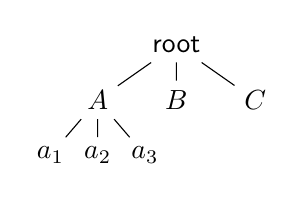
\begin{tikzpicture}[level distance=7mm]
          \tikzstyle{level 1}=[sibling distance=10mm]
          \tikzstyle{level 2}=[sibling distance=6mm]
          \node {$\mathsf{root}$}
              child {node {$A$} child {node {$a_1$}} child {node {$a_2$}} child {node {$a_3$}}}
              child {node {$B$}}
              child {node {$C$}};
      \end{tikzpicture}
  };
  \node [rectangle,draw] (change1) at (5,3) {
      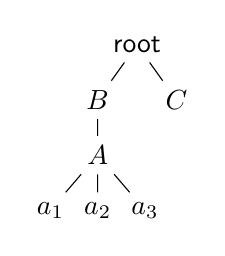
\begin{tikzpicture}[level distance=7mm]
          \tikzstyle{level 1}=[sibling distance=10mm]
          \tikzstyle{level 3}=[sibling distance=6mm]
          \node {$\mathsf{root}$}
              child {node {$B$} child {node {$A$} child {node {$a_1$}} child {node {$a_2$}} child {node {$a_3$}}}}
              child {node {$C$}};
      \end{tikzpicture}
  };
  \node [rectangle,draw] (change2) at (5,0) {
      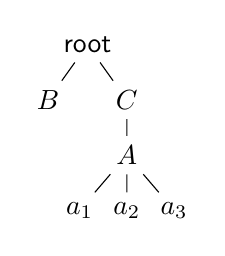
\begin{tikzpicture}[level distance=7mm]
          \tikzstyle{level 1}=[sibling distance=10mm]
          \tikzstyle{level 3}=[sibling distance=6mm]
          \node {$\mathsf{root}$}
              child {node {$B$}}
              child {node {$C$} child {node {$A$} child {node {$a_1$}} child {node {$a_2$}} child {node {$a_3$}}}};
      \end{tikzpicture}
  };
  \node [rectangle,draw,inner sep=3mm] (merge1) at (8.2,3) {?};
  \node [rectangle,draw,inner sep=3mm] (merge2) at (8.2,0) {?};
  \draw [time] (start1.east) -- node [above,text width=2.5cm,text centered,inner ysep=5pt] {Move $A$ to be a child of $B$} (change1.west);
  \draw [time] (change1.east) -- (merge1.west);
  \draw [time] (start2.east) -- node [above,text width=2.5cm,text centered,inner ysep=5pt] {Move $A$ to be a child of $C$} (change2.west);
  \draw [time] (change2.east) -- (merge2.west);
  \draw [network] (6.5,0) to [out=90,in=270] (7.2,3);
  \draw [network] (6.5,3) to [out=270,in=90] (7.2,0);
  \node [rotate=90,blue,font=\footnotesize] at (7.5,1.5) {network communication};
  \path [draw,dotted] (-3.1,1.5) -- (8.7,1.5);
  %%%
  \node [fill=red!15] at (9.83,4.10) {(\emph{a})};
  \node [fill=red!15] at (14.18,4.10) {(\emph{b})};
  \node [fill=red!15] at (9.84,1.10) {(\emph{c})};
  \node [fill=red!15] at (14.15,1.10) {(\emph{d})};
  \node [rectangle,draw] at (10.9,3) {
      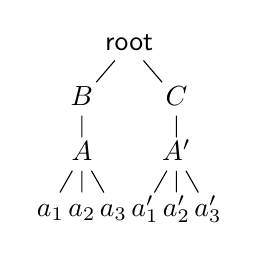
\begin{tikzpicture}[level distance=7mm]
          \tikzstyle{every node}=[text height=5pt,text depth=0pt]
          \tikzstyle{level 1}=[sibling distance=12mm]
          \tikzstyle{level 3}=[sibling distance=4mm]
          \node {$\mathsf{root}$}
              child {node {$B$} child {node {$A$} child {node {$a_1$}} child {node {$a_2$}} child {node {$a_3$}}}}
              child {node {$C$} child {node {$A'$} child {node {$a_1'$}} child {node {$a_2'$}} child {node {$a_3'$}}}};
      \end{tikzpicture}
  };
  \node [rectangle,draw] at (13.5,3) {
      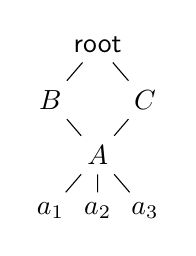
\begin{tikzpicture}[level distance=7mm]
          \tikzstyle{level 1}=[sibling distance=12mm]
          \node at (0,1.4) {$\mathsf{root}$} child {node (b) {$B$}} child {node (c) {$C$}};
          \tikzstyle{level 1}=[sibling distance=6mm]
          \node (a) at (0,0) {$A$} child {node {$a_1$}} child {node {$a_2$}} child {node {$a_3$}};
          \draw (b) -- (a);
          \draw (c) -- (a);
      \end{tikzpicture}
  };
  \node [rectangle,draw] at (10.7,0) {
      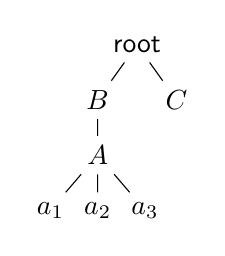
\begin{tikzpicture}[level distance=7mm]
          \tikzstyle{level 1}=[sibling distance=10mm]
          \tikzstyle{level 3}=[sibling distance=6mm]
          \node {$\mathsf{root}$}
              child {node {$B$} child {node {$A$} child {node {$a_1$}} child {node {$a_2$}} child {node {$a_3$}}}}
              child {node {$C$}};
      \end{tikzpicture}
  };
  \node [rectangle,draw] at (13.3,0) {
      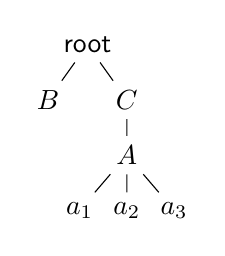
\begin{tikzpicture}[level distance=7mm]
          \tikzstyle{level 1}=[sibling distance=10mm]
          \tikzstyle{level 3}=[sibling distance=6mm]
          \node {$\mathsf{root}$}
              child {node {$B$}}
              child {node {$C$} child {node {$A$} child {node {$a_1$}} child {node {$a_2$}} child {node {$a_3$}}}};
      \end{tikzpicture}
  };
\end{tikzpicture}
\caption{Replica 1 moves $A$ to be a child of $B$, while concurrently replica 2 moves the same node $A$ to be a child of $C$. Boxes (\emph{a}) to (\emph{d}) show possible outcomes after the replicas have communicated and merged their states.}
\label{fig:move-same-item}
\Description{}
\end{figure*}

\begin{figure*}
\centering
\begin{tikzpicture}
  \tikzstyle{time}=[thick,->,gray]
  \tikzstyle{network}=[thick,dashed,blue,-{Stealth[length=3mm]}]
  \node [anchor=east] at (-1.2,3) {Replica 1:};
  \node [anchor=east] at (-1.2,0) {Replica 2:};
  \node [rectangle,draw] (start1) at (0,3) {
      \begin{tikzpicture}[level distance=7mm]
      \node {$\mathsf{root}$} child {node {$A$} child {node {$C$}}} child {node {$B$}};
      \end{tikzpicture}
  };
  \node [rectangle,draw] (start2) at (0,0) {
      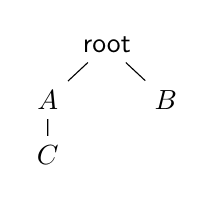
\begin{tikzpicture}[level distance=7mm]
      \node {$\mathsf{root}$} child {node {$A$} child {node {$C$}}} child {node {$B$}};
      \end{tikzpicture}
  };
  \node [rectangle,draw] (change1) at (4.5,3) {
      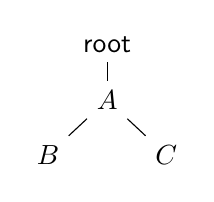
\begin{tikzpicture}[level distance=7mm]
      \node {$\mathsf{root}$} child {node {$A$} child {node {$B$}} child {node {$C$}}};
      \end{tikzpicture}
  };
  \node [rectangle,draw] (change2) at (4.5,0) {
      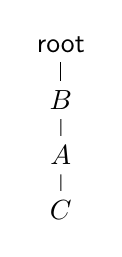
\begin{tikzpicture}[level distance=7mm]
      \node {$\mathsf{root}$} child {node {$B$} child {node {$A$} child {node {$C$}}}};
      \end{tikzpicture}
  };
  \node [rectangle,draw,inner sep=3mm] (merge1) at (8,3) {?};
  \node [rectangle,draw,inner sep=3mm] (merge2) at (8,0) {?};
  \draw [time] (start1.east) -- node [above,text width=2.5cm,text centered,inner ysep=5pt] {Move $B$ to be a child of $A$} (change1.west);
  \draw [time] (change1.east) -- (merge1.west);
  \draw [time] (start2.east) -- node [above,text width=2.5cm,text centered,inner ysep=5pt] {Move $A$ to be a child of $B$} (change2.west);
  \draw [time] (change2.east) -- (merge2.west);
  \draw [network] (6.0,0) to [out=90,in=270] (6.7,3);
  \draw [network] (6.0,3) to [out=270,in=90] (6.7,0);
  \node [rotate=90,blue,font=\footnotesize] at (7.0,1.5) {network communication};
  \path [draw,dotted] (-2.5,1.6) -- (8.5,1.6);
  %%%%%
  \node [rectangle,draw] at (10.95,3) {
      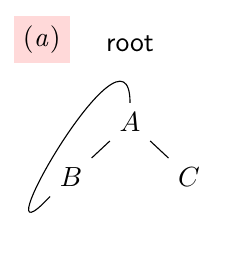
\begin{tikzpicture}[level distance=7mm]
      \useasboundingbox (-1.3,-1.3) rectangle (1,1.2);
      \node [fill=red!15] at (-1.12,1.05) {(\emph{a})};
      \node at (0,1) {$\mathsf{root}$};
      \node (a1) {$A$} child {node (b1) {$B$}} child {node {$C$}};
      \draw (b1.south west) .. controls (-2,-2) and (0,1.5) .. (a1.north);
      \end{tikzpicture}
  };
  \node [rectangle,draw] at (13.8,3) {
      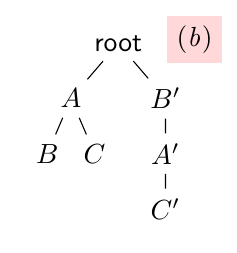
\begin{tikzpicture}[level distance=7mm]
      \useasboundingbox (-1.15,-2.3) rectangle (1.15,0.2);
      \node [fill=red!15] at (0.97,0.05) {(\emph{b})};
      \tikzstyle{level 1}=[sibling distance=12mm]
      \tikzstyle{level 2}=[sibling distance=6mm]
      \node {$\mathsf{root}$}
          child {node {$A$} child {node {$B$}} child {node {$C$}}}
          child {node {$B'$} child {node {$A'$} child {node {$C'$}}}};
      \end{tikzpicture}
  };
  \node [rectangle,draw] (start) at (10.95,0) {
      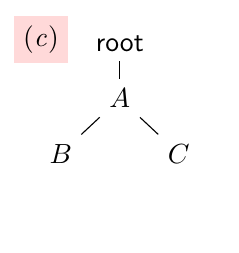
\begin{tikzpicture}[level distance=7mm]
      \useasboundingbox (-1.17,-2.3) rectangle (1.15,0.2);
      \node [fill=red!15] at (-1.00,0.05) {(\emph{c})};
      \node {$\mathsf{root}$} child {node {$A$} child {node {$B$}} child {node {$C$}}};
      \end{tikzpicture}
  };
  \node [rectangle,draw] (right) at (13.8,0) {
      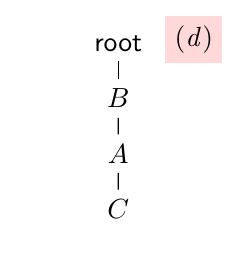
\begin{tikzpicture}[level distance=7mm]
      \useasboundingbox (-1.15,-2.3) rectangle (1.15,0.2);
      \node [fill=red!15] at (0.96,0.05) {(\emph{d})};
      \node {$\mathsf{root}$} child {node {$B$} child {node {$A$} child {node {$C$}}}};
      \end{tikzpicture}
  };
\end{tikzpicture}
\caption{Initially, nodes $A$ and $B$ are siblings. Replica 1 moves $B$ to be a child of $A$, while concurrently replica 2 moves $A$ to be a child of $B$. Boxes (\emph{a}) to (\emph{d}) show possible outcomes after the replicas have communicated and merged their states.}\label{fig:move-cycle}
\Description{Visualisation of trees with concurrent move operations}
\end{figure*}

\begin{figure*}
  \centering
  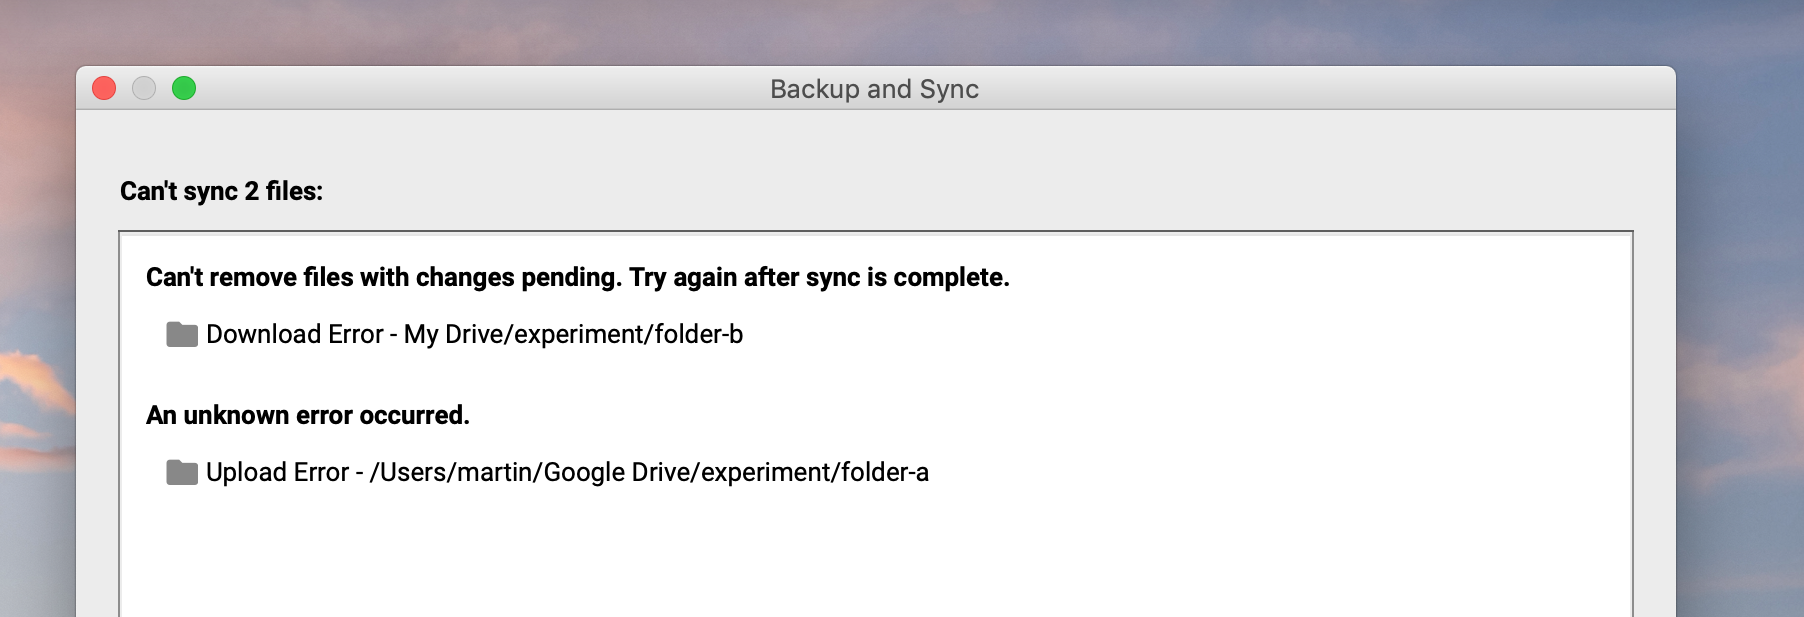
\includegraphics[width=\textwidth,keepaspectratio=true]{gdrive-error.png}
  \caption{Error message produced by Google Drive Backup and Sync on Mac OS as a result of performing the operations shown in Figure~\ref{fig:move-cycle}.}
  \label{fig:gdrive-error}
  \Description{Screenshot showing the errors ``Can't remove files with changes pending. Try again after sync is complete.'' and ``An unknown error occurred.''}
\end{figure*}

\section{Why a move operation is hard}\label{sec:move-is-hard}

Applications that rely on a tree data model often need to move a node from one location to another location within the tree, whereby all children of the moved node move along with it.
For example:
\begin{itemize}
    \item In a filesystem, any file or directory can be moved to a different parent directory.
        Moreover, renaming a file or directory is equivalent to moving it to a new name without changing its parent directory.
    \item In a rich text editor, a paragraph node can be turned into a bullet point.
        In the DOM tree this corresponds to creating a new bullet list node, creating a new bullet point node within it, and then moving the paragraph node to be a child of the new bullet point node.
    \item In presentation software, grouping two graphical objects corresponds to creating a new group node, and then moving the two objects to be children of the new group node.
\end{itemize}
As these operations are so common, it is not obvious why a move operation should be difficult in a replicated setting.
In this section we demonstrate by example some of the problems that arise with replicated trees, before proceeding to our solution in Section~\ref{sec:algorithm}.

\subsection{Concurrent moves of the same node}\label{sec:move-same-item}

The first difficulty arises when a node is moved to a new location on one replica, and concurrently the same node is moved to a different location on a different replica.
This scenario is illustrated in Figure~\ref{fig:move-same-item}, where replica 1 moves node $A$ to be a child of $B$, while concurrently replica 2 moves $A$ to be a child of $C$.
After the replicas communicate these operations to each other, what should the merged state of the tree be?

If a move operation is implemented by deleting the moved subtree from its old location, and then re-creating it at the new location, the merged state will be as shown in Figure~\ref{fig:move-same-item}a: the concurrent moves will duplicate the moved subtree, since each concurrent move independently recreates the subtree in each destination location.
We believe that this duplication is undesirable, since subsequent edits to nodes in the duplicated subtree will apply to only one of the copies.
Two users who believe they are collaborating on the same file may in fact be editing two different copies, which will then become inconsistent with each other.

Rather than duplicating the moved subtree, another possible resolution is for the destination locations of both moves to refer to the same node, as shown in Figure~\ref{fig:move-same-item}b.
However, the result is a DAG, not a tree.
POSIX-compliant filesystems do not allow this outcome, since they allow hardlinks only to files, but not to directories.

In our opinion, the only reasonable outcomes are those shown in Figure~\ref{fig:move-same-item}c and~\ref{fig:move-same-item}d: the moved subtree appears either in replica 1's destination location or in replica 2's destination location, but not in both.
Which one of these two is picked is arbitrary, due to the symmetry between the two replicas.
For example, the ``winning'' location could be picked based on a timestamp in the operations, similarly to the ``last writer wins'' conflict resolution method of Thomas's write rule~\cite{Johnson:1975we}.
All replicas pick the same operation as winner, and effectively ignore the conflicting operation.

We tested this scenario with file sync products Dropbox and Google Drive by concurrently moving the same directory to two different destination directories.\footnote{Experiment setup: we installed the official Mac OS clients for Dropbox and Google Drive on two computers, logged into the same Dropbox/Google accounts, and configured them to each sync a directory on the local filesystem with the corresponding cloud service.
To test concurrent operations, we turned off the network interface on both computers, performed a move operation on the local filesystem of each computer, then reconnected both computers to the Internet and waited for them to sync.}
Dropbox exhibited the undesirable duplication behaviour of Figure~\ref{fig:move-same-item}a, while the outcome on Google Drive was as in Figure~\ref{fig:move-same-item}c/d.

\subsection{Moving a node to be a descendant of itself}\label{sec:move-cycle}

On a filesystem, the destination directory of a move operation must not be a subdirectory of the directory being moved.
For example, if \texttt{b} is a subdirectory of \texttt{a}, then the Unix shell command \texttt{mv a a/b/} will fail with an error.
This restriction is required because allowing this operation would introduce a cycle into the directory graph, and so the filesystem would no longer be a tree.
The same restriction is required in any other tree structure that supports a move operation.

In an unreplicated tree it is easy to prevent cycles being introduced: if the node being moved is an ancestor of the destination node, then the move operation must be rejected.
However, a new problem arises in a replicated setting: different replicas may perform operations that are individually safe, but whose combination leads to a cycle.

One example of such a scenario is illustrated in Figure~\ref{fig:move-cycle}.
Here, replica 1 moves $B$ to be a child of $A$, while concurrently replica 2 moves $A$ to be a child of $B$.
As each replica propagates its operation to the other replica, a careless implementation might end up in the state shown in Figure~\ref{fig:move-cycle}a, in which $A$ and $B$ have become locked in a cycle and detached from the tree.

Another possible resolution is shown in Figure~\ref{fig:move-cycle}b: the nodes involved in the concurrent moves (and their children) could be duplicated, so that both ``$A$ as a child of $B$'' and ``$B$ as a child of $A$'' can exist in the tree.
However, such duplication is undesirable for the same reasons as in Section~\ref{sec:move-same-item}.

In our opinion, the best way of handling the conflicting operations of Figure~\ref{fig:move-cycle} is to choose either Figure~\ref{fig:move-cycle}c or~\ref{fig:move-cycle}d: that is, either the result of applying replica 1's operation and ignoring replica 2's operation, or vice versa.
Like in Section~\ref{sec:move-same-item}, the winning operation can be picked based on an operation timestamp.

As before, we tested this scenario with Google Drive and Dropbox.
In Google Drive, one replica was able to successfully sync with the server, while the other replica displayed the ``unknown error'' message shown in Figure~\ref{fig:gdrive-error}.
The replica in an error state refused to sync the conflicting directory, and its filesystem state remained inconsistent with the other replica.
This error state persisted until the directories on the erroring replica were manually moved to match the state of the other replica.

On the other hand, Dropbox exhibits the duplication behaviour shown in Figure~\ref{fig:move-cycle}b.

\subsection{The impossibility of a highly-available move operation}\label{sec:impossibility}

Najafzadeh et al.~\cite{Najafzadeh:2017vk,Najafzadeh:2018bw} have previously implemented a replicated filesystem with a move operation, and analysed the case of concurrent move operations introducing a cycle, as in Section~\ref{sec:move-cycle}.
Using the CISE ('Cause I'm Strong Enough) proof tool~\cite{DBLP:conf/popl/GotsmanYFNS16,Najafzadeh:2016fi} the authors confirm that it is not sufficient for the replica that generates a move operation to check whether the operation introduces a cycle: like in Figure~\ref{fig:move-cycle}, two concurrent operations may be safe individually, but introduce a cycle when combined.

Najafzadeh et al. propose two solutions to this problem: either to duplicate tree nodes, as in Figure~\ref{fig:move-cycle}b, or to execute a synchronous locking protocol that prevents two move operations from concurrently modifying the same part of the tree.
The downside of a locking protocol is that the move operation is no longer highly available in the presence of network partitions, since it must wait for communication with other replicas.

While these solutions are valid, the authors go on to claim that ``no file system can support an unsynchronised move without anomalies, such as loss or duplication''~\cite{Najafzadeh:2018bw}.
We revisit that claim in this paper: our algorithm does not perform any locking, coordination or synchronisation among replicas, but it nevertheless ensures that the tree invariants are always satisified (in particular, it never introduces cycles), and it never duplicates or loses any tree nodes.
To our knowledge, our algorithm is the first to provide all of these properties simultaneously.
We give a precise specification of our algorithm's consistency properties in Section~\ref{sec:proof}.


\begin{figure*}
\raggedright
\begin{isabellebody}
\internallinenumbers
\isacommand{datatype}\isamarkupfalse%
\ {\isacharparenleft}{\isacharprime}t{\isacharcomma}\ {\isacharprime}n{\isacharcomma}\ {\isacharprime}m{\isacharparenright}\ operation\isanewline
\ \ {\isacharequal}\ Move\ {\isacharparenleft}move{\isacharunderscore}time{\isacharcolon}\ {\isacharprime}t{\isacharparenright}\isanewline
\ \ \ \ \ \ \ \ \ {\isacharparenleft}move{\isacharunderscore}parent{\isacharcolon}\ {\isacharprime}n{\isacharparenright}\isanewline
\ \ \ \ \ \ \ \ \ {\isacharparenleft}move{\isacharunderscore}meta{\isacharcolon}\ {\isacharprime}m{\isacharparenright}\isanewline
\ \ \ \ \ \ \ \ \ {\isacharparenleft}move{\isacharunderscore}child{\isacharcolon}\ {\isacharprime}n{\isacharparenright}\isanewline
\isanewline
\isacommand{datatype}\isamarkupfalse%
\ {\isacharparenleft}{\isacharprime}t{\isacharcomma}\ {\isacharprime}n{\isacharcomma}\ {\isacharprime}m{\isacharparenright}\ log{\isacharunderscore}op\isanewline
\ \ {\isacharequal}\ LogMove\ {\isacharparenleft}log{\isacharunderscore}time{\isacharcolon}\ {\isacharprime}t{\isacharparenright}\isanewline
\ \ \ \ \ \ \ \ \ \ \ \ {\isacharparenleft}old{\isacharunderscore}parent{\isacharcolon}\ {\isacartoucheopen}{\isacharparenleft}{\isacharprime}n\ {\isasymtimes}\ {\isacharprime}m{\isacharparenright}\ option{\isacartoucheclose}{\isacharparenright}\isanewline
\ \ \ \ \ \ \ \ \ \ \ \ {\isacharparenleft}new{\isacharunderscore}parent{\isacharcolon}\ {\isacharprime}n{\isacharparenright}\isanewline
\ \ \ \ \ \ \ \ \ \ \ \ {\isacharparenleft}log{\isacharunderscore}meta{\isacharcolon}\ {\isacharprime}m{\isacharparenright}\isanewline
\ \ \ \ \ \ \ \ \ \ \ \ {\isacharparenleft}log{\isacharunderscore}child{\isacharcolon}\ {\isacharprime}n{\isacharparenright}\isanewline
\isanewline
\isacommand{type{\isacharunderscore}synonym}\isamarkupfalse%
\ {\isacharparenleft}{\isacharprime}t{\isacharcomma}\ {\isacharprime}n{\isacharcomma}\ {\isacharprime}m{\isacharparenright}\ state\ {\isacharequal}\ {\isacartoucheopen}{\isacharparenleft}{\isacharprime}t{\isacharcomma}\ {\isacharprime}n{\isacharcomma}\ {\isacharprime}m{\isacharparenright}\ log{\isacharunderscore}op\ list\ {\isasymtimes}\ {\isacharparenleft}{\isacharprime}n\ {\isasymtimes}\ {\isacharprime}m\ {\isasymtimes}\ {\isacharprime}n{\isacharparenright}\ set{\isacartoucheclose}\isanewline
\isanewline
\isacommand{definition}\isamarkupfalse%
\ get{\isacharunderscore}parent\ {\isacharcolon}{\isacharcolon}\ {\isacartoucheopen}{\isacharparenleft}{\isacharprime}n\ {\isasymtimes}\ {\isacharprime}m\ {\isasymtimes}\ {\isacharprime}n{\isacharparenright}\ set\ {\isasymRightarrow}\ {\isacharprime}n\ {\isasymRightarrow}\ {\isacharparenleft}{\isacharprime}n\ {\isasymtimes}\ {\isacharprime}m{\isacharparenright}\ option{\isacartoucheclose}\ \isakeyword{where}\isanewline
\ \ {\isacartoucheopen}get{\isacharunderscore}parent\ tree\ child\ {\isasymequiv}\isanewline
\ \ \ \ \ if\ {\isasymexists}{\isacharbang}parent{\isachardot}\ {\isasymexists}{\isacharbang}meta{\isachardot}\ {\isacharparenleft}parent{\isacharcomma}\ meta{\isacharcomma}\ child{\isacharparenright}\ {\isasymin}\ tree\ then\isanewline
\ \ \ \ \ \ \ Some\ {\isacharparenleft}THE\ {\isacharparenleft}parent{\isacharcomma}\ meta{\isacharparenright}{\isachardot}\ {\isacharparenleft}parent{\isacharcomma}\ meta{\isacharcomma}\ child{\isacharparenright}\ {\isasymin}\ tree{\isacharparenright}\isanewline
\ \ \ \ \ else\ None{\isacartoucheclose}\isanewline
\isanewline
\isacommand{inductive}\isamarkupfalse%
\ ancestor\ {\isacharcolon}{\isacharcolon}\ {\isacartoucheopen}{\isacharparenleft}{\isacharprime}n\ {\isasymtimes}\ {\isacharprime}m\ {\isasymtimes}\ {\isacharprime}n{\isacharparenright}\ set\ {\isasymRightarrow}\ {\isacharprime}n\ {\isasymRightarrow}\ {\isacharprime}n\ {\isasymRightarrow}\ bool{\isacartoucheclose}\ \isakeyword{where}\isanewline
\ \ {\isacartoucheopen}{\isasymlbrakk}{\isacharparenleft}parent{\isacharcomma}\ meta{\isacharcomma}\ child{\isacharparenright}\ {\isasymin}\ tree{\isasymrbrakk}\ {\isasymLongrightarrow}\ ancestor\ tree\ parent\ child{\isacartoucheclose}\ {\isacharbar}\isanewline
\ \ {\isacartoucheopen}{\isasymlbrakk}{\isacharparenleft}parent{\isacharcomma}\ meta{\isacharcomma}\ child{\isacharparenright}\ {\isasymin}\ tree{\isacharsemicolon}\ ancestor\ tree\ anc\ parent{\isasymrbrakk}\ {\isasymLongrightarrow}\ ancestor\ tree\ anc\ child{\isacartoucheclose}\isanewline
\isanewline
\isacommand{fun}\isamarkupfalse%
\ do{\isacharunderscore}op\ {\isacharcolon}{\isacharcolon}\ {\isacartoucheopen}{\isacharparenleft}{\isacharprime}t{\isacharcomma}\ {\isacharprime}n{\isacharcomma}\ {\isacharprime}m{\isacharparenright}\ operation\ {\isasymtimes}\ {\isacharparenleft}{\isacharprime}n\ {\isasymtimes}\ {\isacharprime}m\ {\isasymtimes}\ {\isacharprime}n{\isacharparenright}\ set\ {\isasymRightarrow}\isanewline
\ \ \ \ \ \ \ \ \ \ \ \ \ \ {\isacharparenleft}{\isacharprime}t{\isacharcomma}\ {\isacharprime}n{\isacharcomma}\ {\isacharprime}m{\isacharparenright}\ log{\isacharunderscore}op\ {\isasymtimes}\ {\isacharparenleft}{\isacharprime}n\ {\isasymtimes}\ {\isacharprime}m\ {\isasymtimes}\ {\isacharprime}n{\isacharparenright}\ set{\isacartoucheclose}\ \isakeyword{where}\isanewline
\ \ {\isacartoucheopen}do{\isacharunderscore}op\ {\isacharparenleft}Move\ t\ newp\ m\ c{\isacharcomma}\ tree{\isacharparenright}\ {\isacharequal}\isanewline
\ \ \ \ \ {\isacharparenleft}LogMove\ t\ {\isacharparenleft}get{\isacharunderscore}parent\ tree\ c{\isacharparenright}\ newp\ m\ c{\isacharcomma}\isanewline
\ \ \ \ \ \ if\ ancestor\ tree\ c\ newp\ {\isasymor}\ c\ {\isacharequal}\ newp\ then\ tree\isanewline
\ \ \ \ \ \ else\ {\isacharbraceleft}{\isacharparenleft}p{\isacharprime}{\isacharcomma}\ m{\isacharprime}{\isacharcomma}\ c{\isacharprime}{\isacharparenright}\ {\isasymin}\ tree{\isachardot}\ c{\isacharprime}\ {\isasymnoteq}\ c{\isacharbraceright}\ {\isasymunion}\ {\isacharbraceleft}{\isacharparenleft}newp{\isacharcomma}\ m{\isacharcomma}\ c{\isacharparenright}{\isacharbraceright}{\isacharparenright}{\isacartoucheclose}\isanewline
\isanewline
\isacommand{fun}\isamarkupfalse%
\ undo{\isacharunderscore}op\ {\isacharcolon}{\isacharcolon}\ {\isacartoucheopen}{\isacharparenleft}{\isacharprime}t{\isacharcomma}\ {\isacharprime}n{\isacharcomma}\ {\isacharprime}m{\isacharparenright}\ log{\isacharunderscore}op\ {\isasymtimes}\ {\isacharparenleft}{\isacharprime}n\ {\isasymtimes}\ {\isacharprime}m\ {\isasymtimes}\ {\isacharprime}n{\isacharparenright}\ set\ {\isasymRightarrow}\ {\isacharparenleft}{\isacharprime}n\ {\isasymtimes}\ {\isacharprime}m\ {\isasymtimes}\ {\isacharprime}n{\isacharparenright}\ set{\isacartoucheclose}\ \isakeyword{where}\isanewline
\ \ {\isacartoucheopen}undo{\isacharunderscore}op\ {\isacharparenleft}LogMove\ t\ None\ newp\ m\ c{\isacharcomma}\ tree{\isacharparenright}\ {\isacharequal}\ {\isacharbraceleft}{\isacharparenleft}p{\isacharprime}{\isacharcomma}\ m{\isacharprime}{\isacharcomma}\ c{\isacharprime}{\isacharparenright}\ {\isasymin}\ tree{\isachardot}\ c{\isacharprime}\ {\isasymnoteq}\ c{\isacharbraceright}{\isacartoucheclose}\ {\isacharbar}\isanewline
\ \ {\isacartoucheopen}undo{\isacharunderscore}op\ {\isacharparenleft}LogMove\ t\ {\isacharparenleft}Some\ {\isacharparenleft}oldp{\isacharcomma}\ oldm{\isacharparenright}{\isacharparenright}\ newp\ m\ c{\isacharcomma}\ tree{\isacharparenright}\ {\isacharequal}\isanewline
\ \ \ \ \ {\isacharbraceleft}{\isacharparenleft}p{\isacharprime}{\isacharcomma}\ m{\isacharprime}{\isacharcomma}\ c{\isacharprime}{\isacharparenright}\ {\isasymin}\ tree{\isachardot}\ c{\isacharprime}\ {\isasymnoteq}\ c{\isacharbraceright}\ {\isasymunion}\ {\isacharbraceleft}{\isacharparenleft}oldp{\isacharcomma}\ oldm{\isacharcomma}\ c{\isacharparenright}{\isacharbraceright}{\isacartoucheclose}\isanewline
\isanewline
\isacommand{fun}\isamarkupfalse%
\ redo{\isacharunderscore}op\ {\isacharcolon}{\isacharcolon}\ {\isacartoucheopen}{\isacharparenleft}{\isacharprime}t{\isacharcomma}\ {\isacharprime}n{\isacharcomma}\ {\isacharprime}m{\isacharparenright}\ log{\isacharunderscore}op\ {\isasymRightarrow}\ {\isacharparenleft}{\isacharprime}t{\isacharcomma}\ {\isacharprime}n{\isacharcomma}\ {\isacharprime}m{\isacharparenright}\ state\ {\isasymRightarrow}\ {\isacharparenleft}{\isacharprime}t{\isacharcomma}\ {\isacharprime}n{\isacharcomma}\ {\isacharprime}m{\isacharparenright}\ state{\isacartoucheclose}\ \isakeyword{where}\isanewline
\ \ {\isacartoucheopen}redo{\isacharunderscore}op\ {\isacharparenleft}LogMove\ t\ {\isacharunderscore}\ p\ m\ c{\isacharparenright}\ {\isacharparenleft}ops{\isacharcomma}\ tree{\isacharparenright}\ {\isacharequal}\isanewline
\ \ \ \ \ {\isacharparenleft}let\ {\isacharparenleft}op{\isadigit{2}}{\isacharcomma}\ tree{\isadigit{2}}{\isacharparenright}\ {\isacharequal}\ do{\isacharunderscore}op\ {\isacharparenleft}Move\ t\ p\ m\ c{\isacharcomma}\ tree{\isacharparenright}\isanewline
\ \ \ \ \ \ in\ {\isacharparenleft}op{\isadigit{2}}\ {\isacharhash}\ ops{\isacharcomma}\ tree{\isadigit{2}}{\isacharparenright}{\isacharparenright}{\isacartoucheclose}\isanewline
\isanewline
\isacommand{fun}\isamarkupfalse%
\ apply{\isacharunderscore}op\ {\isacharcolon}{\isacharcolon}\ {\isacartoucheopen}{\isacharparenleft}{\isacharprime}t{\isacharcolon}{\isacharcolon}{\isacharbraceleft}linorder{\isacharbraceright}{\isacharcomma}\ {\isacharprime}n{\isacharcomma}\ {\isacharprime}m{\isacharparenright}\ operation\ {\isasymRightarrow}\isanewline
\ \ \ \ \ \ \ \ \ \ \ \ \ \ \ \ \ \ {\isacharparenleft}{\isacharprime}t{\isacharcomma}\ {\isacharprime}n{\isacharcomma}\ {\isacharprime}m{\isacharparenright}\ state\ {\isasymRightarrow}\ {\isacharparenleft}{\isacharprime}t{\isacharcomma}\ {\isacharprime}n{\isacharcomma}\ {\isacharprime}m{\isacharparenright}\ state{\isacartoucheclose}\ \isakeyword{where}\isanewline
\ \ {\isacartoucheopen}apply{\isacharunderscore}op\ op{\isadigit{1}}\ {\isacharparenleft}{\isacharbrackleft}{\isacharbrackright}{\isacharcomma}\ tree{\isadigit{1}}{\isacharparenright}\ {\isacharequal}\isanewline
\ \ \ \ \ {\isacharparenleft}let\ {\isacharparenleft}op{\isadigit{2}}{\isacharcomma}\ tree{\isadigit{2}}{\isacharparenright}\ {\isacharequal}\ do{\isacharunderscore}op\ {\isacharparenleft}op{\isadigit{1}}{\isacharcomma}\ tree{\isadigit{1}}{\isacharparenright}\isanewline
\ \ \ \ \ \ in\ {\isacharparenleft}{\isacharbrackleft}op{\isadigit{2}}{\isacharbrackright}{\isacharcomma}\ tree{\isadigit{2}}{\isacharparenright}{\isacharparenright}{\isacartoucheclose}\ {\isacharbar}\isanewline
\ \ {\isacartoucheopen}apply{\isacharunderscore}op\ op{\isadigit{1}}\ {\isacharparenleft}logop\ {\isacharhash}\ ops{\isacharcomma}\ tree{\isadigit{1}}{\isacharparenright}\ {\isacharequal}\isanewline
\ \ \ \ \ {\isacharparenleft}if\ move{\isacharunderscore}time\ op{\isadigit{1}}\ {\isacharless}\ log{\isacharunderscore}time\ logop\isanewline
\ \ \ \ \ \ then\ redo{\isacharunderscore}op\ logop\ {\isacharparenleft}apply{\isacharunderscore}op\ op{\isadigit{1}}\ {\isacharparenleft}ops{\isacharcomma}\ undo{\isacharunderscore}op\ {\isacharparenleft}logop{\isacharcomma}\ tree{\isadigit{1}}{\isacharparenright}{\isacharparenright}{\isacharparenright}\isanewline
\ \ \ \ \ \ else\ let\ {\isacharparenleft}op{\isadigit{2}}{\isacharcomma}\ tree{\isadigit{2}}{\isacharparenright}\ {\isacharequal}\ do{\isacharunderscore}op\ {\isacharparenleft}op{\isadigit{1}}{\isacharcomma}\ tree{\isadigit{1}}{\isacharparenright}\ in\ {\isacharparenleft}op{\isadigit{2}}\ {\isacharhash}\ logop\ {\isacharhash}\ ops{\isacharcomma}\ tree{\isadigit{2}}{\isacharparenright}{\isacharparenright}{\isacartoucheclose}\isanewline
\isanewline
\isacommand{definition}\isamarkupfalse%
\ apply{\isacharunderscore}ops\ {\isacharcolon}{\isacharcolon}\ {\isacartoucheopen}{\isacharparenleft}{\isacharprime}t{\isacharcolon}{\isacharcolon}{\isacharbraceleft}linorder{\isacharbraceright}{\isacharcomma}\ {\isacharprime}n{\isacharcomma}\ {\isacharprime}m{\isacharparenright}\ operation\ list\ {\isasymRightarrow}\ {\isacharparenleft}{\isacharprime}t{\isacharcomma}\ {\isacharprime}n{\isacharcomma}\ {\isacharprime}m{\isacharparenright}\ state{\isacartoucheclose}\ \isakeyword{where}\isanewline
\ \ {\isacartoucheopen}apply{\isacharunderscore}ops\ ops\ {\isasymequiv}\ foldl\ {\isacharparenleft}{\isasymlambda}state\ oper{\isachardot}\ apply{\isacharunderscore}op\ oper\ state{\isacharparenright}\ {\isacharparenleft}{\isacharbrackleft}{\isacharbrackright}{\isacharcomma}\ {\isacharbraceleft}{\isacharbraceright}{\isacharparenright}\ ops{\isacartoucheclose}\isanewline
\isanewline
\isacommand{definition}\isamarkupfalse%
\ unique{\isacharunderscore}parent\ {\isacharcolon}{\isacharcolon}\ {\isacartoucheopen}{\isacharparenleft}{\isacharprime}n\ {\isasymtimes}\ {\isacharprime}m\ {\isasymtimes}\ {\isacharprime}n{\isacharparenright}\ set\ {\isasymRightarrow}\ bool{\isacartoucheclose}\ \isakeyword{where}\isanewline
\ \ {\isacartoucheopen}unique{\isacharunderscore}parent\ tree\ {\isasymequiv}\ {\isacharparenleft}{\isasymforall}p{\isadigit{1}}\ p{\isadigit{2}}\ m{\isadigit{1}}\ m{\isadigit{2}}\ c{\isachardot}\ {\isacharparenleft}p{\isadigit{1}}{\isacharcomma}\ m{\isadigit{1}}{\isacharcomma}\ c{\isacharparenright}\ {\isasymin}\ tree\ {\isasymand}\ {\isacharparenleft}p{\isadigit{2}}{\isacharcomma}\ m{\isadigit{2}}{\isacharcomma}\ c{\isacharparenright}\ {\isasymin}\ tree\ {\isasymlongrightarrow}\ p{\isadigit{1}}\ {\isacharequal}\ p{\isadigit{2}}\ {\isasymand}\ m{\isadigit{1}}\ {\isacharequal}\ m{\isadigit{2}}{\isacharparenright}{\isacartoucheclose}\isanewline%
\isanewline
\isacommand{definition}\isamarkupfalse%
\ acyclic\ {\isacharcolon}{\isacharcolon}\ {\isacartoucheopen}{\isacharparenleft}{\isacharprime}n\ {\isasymtimes}\ {\isacharprime}m\ {\isasymtimes}\ {\isacharprime}n{\isacharparenright}\ set\ {\isasymRightarrow}\ bool{\isacartoucheclose}\ \isakeyword{where}\isanewline
\ \ {\isacartoucheopen}acyclic\ tree\ {\isasymequiv}\ {\isacharparenleft}{\isasymnexists}n{\isachardot}\ ancestor\ tree\ n\ n{\isacharparenright}{\isacartoucheclose}
\end{isabellebody}
\caption{The move operation algorithm, implemented in the Isabelle/HOL language.}
\label{fig:code}
\Description{The move operation algorithm, implemented in the Isabelle/HOL language.}
\end{figure*}

\section{The replicated move operation}\label{sec:algorithm}

We now introduce our algorithm for a replicated tree data structure that supports a move operation.
We model each replica as a state machine that transitions from one state to the next by applying an operation.
The algorithm is executed independently on each replica with no shared memory between replicas.

When the user makes a change to the tree, that change is expressed by generating an operation on their local replica.
We assume the existence of a messaging middleware that copies operations between replicas, so that eventually every operation is applied on every replica, provided that network partitions are of a finite duration.
This middleware may deliver operations in any order.
Operations received from a remote replica are applied in exactly the same way as operations generated by a local user.

The key consistency property of our algorithm is \emph{convergence}: that is, whenever any two replicas have applied the same set of operations, then they must be in the same state---even if the operations were applied in a different order on different replicas.
We prove this in Section~\ref{sec:proof} by showing that with our algorithm, applying operations is commutative.

Figure~\ref{fig:code} gives the full source code for our algorithm, implemented using the Isabelle/HOL language~\cite{DBLP:conf/tphol/WenzelPN08}.
We choose this language because it combines the conciseness of pseudocode with the precision of mathematical notation.
It supports formal reasoning, allowing us to prove the correctness of the algorithm (Section~\ref{sec:proof}), and it also allows executable code to be exported to common functional programming languages such as Scala, Haskell, OCaml, or Standard ML (Section~\ref{sec:evaluation}).

In this section we walk through the code in Figure~\ref{fig:code} step by step, explaining features of the Isabelle/HOL syntax as we encounter them.
For additional background on the language, standard documentation is available~\cite{DBLP:books/sp/NipkowK14}.

\subsection{Operations and trees}\label{sec:ops-trees}

We define only one kind of operation: \isa{Move t p m c} (Figure~\ref{fig:code}, lines 1--5).
A move operation is a record consisting of four fields: a timestamp \isa{t} of type \isa{'t}, a parent node \isa{p} of type \isa{'n}, a metadata field \isa{m} of type \isa{'m}, and a child node \isa{c} of type \isa{'n}.
Here, \isa{'t}, \isa{'n} and \isa{'m} are \emph{type variables} that can be \emph{substituted} for arbitrary types; our only requirement is that timestamps \isa{'t} are globally unique and have an associated total order.
Concretely, Lamport timestamps~\cite{Lamport:1978jq} would meet these requirements.

The meaning of an operation \isa{Move t p m c} is that at time \isa{t}, the child node \isa{c} is moved to be a child of parent node \isa{p}.
The operation does not specify the old location of \isa{c}; the algorithm simply ``steals'' \isa{c} from wherever it is currently located in the tree, and moves it to \isa{p}.
If \isa{c} does not currently exist in the tree, it is created as a child of \isa{p}.
For this reason we do not need a separate operation type to create tree nodes: simply performing a move with a fresh child node \isa{c} is sufficient to create \isa{c}.
Moreover, we do not define a remove operation: instead, we can designate a particular tree node as the ``trash'', and perform deletion of a node \isa{c} by moving \isa{c} to be a child of the trash node.

The metadata field \isa{m} in a move operation allows additional information to be associated with the parent-child relationship of \isa{p} and \isa{c}.
For example, in a filesystem, the parent and child would be the inodes of a directory and a file within it, respectively, and the metadata would contain the filename of the child.
Thus, a file with inode \isa{c} can be renamed by performing a \isa{Move t p m c}, where the new parent directory \isa{p} is the unchanged inode of the existing parent directory, but the metadata \isa{m} contains the new filename.

When users want to make changes to the tree on their local replica, they generate new \isa{Move t p m c} operations for these changes, and apply these operations to their local replica.
The timestamp \isa{t} of each operation must be globally unique; the other fields \isa{p}, \isa{m} and \isa{c} can be chosen freely.

We can now represent the tree as a set of \isa{(parent, meta, child)} triples, denoted in Isabelle as \isa{('n {\isasymtimes} 'm {\isasymtimes} 'n) set}.
When we have \isa{(p, m, c) {\isasymin} tree}, that means \isa{c} is a child of \isa{p} in the tree, with associated metadata \isa{m}.
Given a \isa{tree}, we can move the child \isa{c} to a new parent \isa{p}, with associated metadata \isa{m}, as follows:
\begin{quote}
\isa{\{(p', m', c') {\isasymin} tree. c' {\isasymnoteq} c\} {\isasymunion} \{(p, m, c)\}}
\end{quote}
That is, we remove any existing parent-child relationship for \isa{c} from the set \isa{tree}, and then add \isa{\{(p, m, c)\}} to represent the new parent-child relationship.
This expression appears on lines 31 and 36 of Figure~\ref{fig:code}, as we shall explain shortly.

\subsection{Replica state and operation log}\label{sec:state-log}

In order to correctly apply move operations, a replica needs to maintain not only the current state of the tree, but also an \emph{operation log}.
The log is a list of \isa{LogMove} records in descending timestamp order.
A \isa{LogMove t oldp p m c} record (lines 7--12) is similar to a record \isa{Move t p m c}; the only difference is that the \isa{LogMove} has an additional field \isa{oldp} of type \isa{('n {\isasymtimes} 'm) option}.
This \isa{option} type means the field can either take the value \isa{None} (intuitively similar to null), or a pair of an inode and a metadata field.

When a replica applies a \isa{Move} operation to its tree, it also records a corresponding \isa{LogMove} operation in its log.
The \isa{t}, \isa{p}, \isa{m} and \isa{c} fields are taken directly from the \isa{Move} record, while the \isa{oldp} field is filled in based on the state of the tree before the move.
If \isa{c} did not exist in the tree prior to the move, \isa{oldp} is set to \isa{None}.
Otherwise, \isa{oldp} records the previous parent and metadata of \isa{c}, that is: if there exists a \isa{p'} and \isa{m'} such that \isa{(p', m', c) {\isasymin} tree}, then \isa{oldp} is set to \isa{Some (p', m')}.
This logic is performed by the \isa{get\_parent} function (lines 16--20).

In the first line of \isa{get\_parent}, the expression between \isa{::} and \textbf{where} is the type signature of the function, in this case:
\begin{quote}
\isa{('n {\isasymtimes} 'm {\isasymtimes} 'n) set {\isasymRightarrow} 'n {\isasymRightarrow} ('n {\isasymtimes} 'm) option}
\end{quote}
This signature denotes a function that takes two arguments: a tree \isa{('n {\isasymtimes} 'm {\isasymtimes} 'n) set} and a node \isa{'n}.
It then returns a \isa{('n {\isasymtimes} 'm) option}.
\isa{{\isasymexists}!x} means ``there exists a unique value \isa{x} such that\dots'', whilst $\isa{THE}\ \isa{x}. \ldots$ means ``\emph{choose} the unique value \isa{x} such that\ldots''.

In line 14 we define the datatype for the state of a replica: a pair \isa{(log, tree)} where \isa{log} is a list of \isa{LogMove} records, and \isa{tree} is a set of \isa{(parent, meta, child)} triples as before.

\subsection{Preventing cycles}\label{sec:prevent-cycles}

Recall from Section~\ref{sec:move-cycle} that in order to prevent a cycle being introduced, the node being moved must not be an ancestor of the destination node.
To implement this in Figure~\ref{fig:code}, we first define the \isa{ancestor} relation in lines 22--24.
This relation is the transitive closure of the parent-child relation of a tree: if \isa{(p, m, c) {\isasymin} tree} then \isa{p} is an ancestor of \isa{c} (line 23); moreover, if \isa{(p, m, c) {\isasymin} tree} and \isa{a} is an ancestor of \isa{p}, then \isa{a} is also an ancestor of \isa{c} (line 24).
The \textbf{inductive} keyword indicates that this recursive definition is iterated until a fixed point (the least) is reached.

The \isa{do\_op} function (lines 26--31) now performs the actual work of applying a move operation.
This function takes as argument a pair consisting of a \isa{Move} operation and the current tree, and it returns a pair consisting of a \isa{LogMove} operation (which will be added to the log) and an updated tree.
In line 29, the \isa{LogMove} record is constructed as described in Section~\ref{sec:state-log}, obtaining the prior parent and metadata of \isa{c} using the \isa{get\_parent} function.

Line 30 performs the check that ensures no cycles are introduced: if \isa{ancestor tree c newp}, i.e.\ if the node \isa{c} is being moved, and \isa{c} is an ancestor of the new parent \isa{newp}, then the tree is returned unmodified---in other words, the operation is ignored.
Similarly, if \isa{c = newp}, the operation is also ignored.
Otherwise (line 31), the tree is updated by removing \isa{c} from its existing parent, if any, and adding the new parent-child relationship \isa{(newp, m, c)} to the tree.

\subsection{Applying operations in any order}\label{sec:applying}

The \isa{do\_op} function is sufficient for applying operations if all replicas apply operations in the same order.
However, in an optimistic replication setting, each replica may apply the operations in a different order, and we need to ensure that the replica state nevertheless converges towards a consistent state.
This goal is accomplished by the \isa{undo\_op}, \isa{redo\_op}, and \isa{apply\_op} functions (lines 33--51).

The intuition behind these functions is as follows: when a replica needs to apply an operation with timestamp \isa{t}, it first undoes the effect of any operations with a timestamp greater than \isa{t}, then performs the new operation, and finally re-applies the previously undone operations.
The result of this procedure is that the state of the tree is as if the operations had all been applied in order of increasing timestamp, even though in fact they might have been applied in any order.

The \isa{apply\_op} function (lines 43--51) takes two arguments: a \isa{Move} operation to apply and the current replica state; and it returns the new replica state.
The constraint \isa{'t::\{linorder\}} in the type signature indicates that timestamps \isa{'t} are instances of \isa{linorder} type class, and timestamps can therefore be compared with the \isa{<} operator defining a total order.
This comparison occurs on line 49.

Recall that the replica state includes the operation log (line 14), and we use this log to perform the undo-do-redo cycle.
Lines 45--47 handle the case where the log is empty: in this case, we simply perform the operation using \isa{do\_op}, and return the new tree along with a log containing a single \isa{LogMove} record.

If the log is nonempty (line 48), we take \isa{logop} to be the first element of the log, and \isa{ops} to be the rest.
(The hash character in \isa{logop {\isacharhash} ops} is the \emph{cons} operator that adds one element to the head of a list.)
If the timestamp of \isa{logop} is greater than the timestamp of the new operation (line 49) we first undo \isa{logop} with \isa{undo\_op}, then recursively apply the new operation to the remaining log, and finally reapply \isa{logop} with \isa{redo\_op} (line 50).
Otherwise we perform the operation using \isa{do\_op}, and add the corresponding \isa{LogMove} record as the head of the log (line 51).

This logic ensures that the log is maintained in descending timestamp order, with the greatest timestamp at the head.
\isa{undo\_op} (lines 33--36) inverts the effect of a previous move operation by restoring the prior parent and metadata that were recorded in the \isa{LogMove}'s additional field.
\isa{redo\_op} (lines 38--41) uses \isa{do\_op} to perform an operation again and recomputes the \isa{LogMove} record (which might have changed due to the effect of the new operation with a lower timestamp).

\subsection{Handling conflicts}\label{sec:conflicts}

The consequence of performing the undo-do-redo cycle is that, effectively, the state of the tree is as if all operations had been applied using \isa{do\_op} in increasing timestamp order, regardless of the order in which they were actually applied.
This provides a clear approach to the handling of conflicts:
\begin{itemize}
    \item If two operations concurrently move the same node, then the ``winning'' operation is the one with the higher timestamp.
        This is the case because, if the operations are applied in increasing timestamp order, the node being moved is first moved to the parent indicated by the operation with the lower timestamp, and then moved again to the parent indicated by the operation with the higher timestamp.
        Since move operations do not specify the old location of a node, but only the new location, this sequential execution of concurrent operations is well-defined.
    \item If two operations would introduce a cycle when combined, as in Section~\ref{sec:move-cycle}, then the operation with the greater timestamp is ignored.
        This is the case because \isa{do\_op} checks for cycles based on the tree created by all operations with a lower timestamp.
        The lower of two conflicting operations will take effect, since that operation by itself is safe.
        When the higher-timestamped operation is applied, \isa{do\_op} detects that it would introduce a cycle, and therefore ignores the operation.
\end{itemize}

Note that the safety of an operation (whether or not it would introduce a cycle) may change as subsequent operations with lower timestamps are applied.
For example, an operation may initially be regarded as safe, and then be reclassified as unsafe after applying a conflicting operation with a lower timestamp.
The opposite is also possible: an operation previously regarded as unsafe may become safe through the application of a lower-timestamped operation that removes the risk of introducing a cycle.
For this reason, the operation log must include all operations, even those that have no effect on the tree.

One final type of conflict that we have not discussed so far is multiple child nodes with the same parent and the same metadata.
For example, in a filesystem, two users could concurrently create files with the same name in the same directory.
Our algorithm does not take any measures to prevent such conflict, but simply retains both child nodes.
In practice, the filename collision would be resolved by making the filenames distinct, e.g.\ by appending a replica identifier to the filenames.

\subsection{Algorithm extensions}\label{sec:extensions}

The algorithm as specified in Figure~\ref{fig:code} retains operations in the log indefinitely, so the memory/storage use grows without bound.
However, in practice it is easy to truncate the log, because \isa{apply\_op} only examines the prefix of operations whose timestamp is greater than that of the operation being applied.
Thus, once it is known that all future operations will have a timestamp greater than $t$, then all operations with timestamp $t$ or less can be discarded from the log.
In this case, we say that $t$ is \emph{causally stable}~\cite{Baquero:2014ed}.

We can determine causal stability in a system where the set of replicas is known, where each replica generates operations with monotonically increasing timestamps, and where the communication link between any pair of replicas is FIFO (messages are received in the order in which they are sent, as implemented e.g. by TCP).
In this case, each replica can keep track of the most recent timestamp it has seen from all replicas (including its own), and the minimum of these timestamps is the causally stable threshold.

Another useful extension of the tree algorithm is to allow children within the same branch node to have an ordering.
For example, in a graphics application, the order of nodes determines visibility (objects that are ``further back'' may be obscured by objects that are ``closer to the front'').
This can be implemented by maintaining a separate list CRDT for each branch node, e.g.\ using RGA~\cite{Roh:2011dw}, Treedoc~\cite{Preguica:2009fz}, Logoot~\cite{Weiss:2010hx}, or LSEQ~\cite{Nedelec:2013ky}.
These algorithms assign a unique identifier to each element of the list, and this unique identifier can be included in the metadata field of move operations in order to determine the order of children of the same parent node.

This approach to determining ordering also easily supports reordering of child nodes within a parent, e.g.\ to implement the ``bring to front'' and ``send to back'' feature of applications like PowerPoint.
To move a node to a different position in a list, we use the list CRDT to generate a new identifier at the desired position in the sequence.
Then we perform a move operation in which the parent node is unchanged, but the metadata is updated to include this new identifier.

% - No Synchronisation or consensus required. Available in the sense of CAP
% - Rely only on uniqueness of node IDs, e.g. inode numbers
% - Composing JSON/XML tree by using list datatype
% - Location is Lww register. Concurrent move does not duplicate
% - Unlike NFS, can work offline 
% - Garbage collection: discard causally stable prefix

\section{Proof of correctness}\label{sec:proof}

We now discuss the correctness properties of the algorithm from Section~\ref{sec:algorithm}.
All theorems stated here have been formally proved and mechanically checked using Isabelle.
For space reasons we give only a brief sketch of the proofs in this paper, but the full details can be found in the open source Isabelle files of our proof development.\footnote{\url{https://github.com/trvedata/move-op}}

To reason about the state of a replica we define the function \isa{apply\_ops} on lines 53--54 of Figure~\ref{fig:code}.
It takes a list of operations \isa{ops} and returns the state of a replica after it has applied all the operations in \isa{ops}.
The \isa{apply\_ops} function works by starting in the initial state \isa{([], \{\})} consisting of the empty operation log \isa{[]} and the empty tree \isa{\{\}}, and then applying the operations one by one to the state using the \isa{apply\_op} function (introduced in Section~\ref{sec:applying}).
The \isa{foldl} function from Isabelle's standard library performs the iteration over the list of operations.

\subsection{Tree invariants}\label{sec:tree-invariants}

A tree is an acyclic graph in which every node has exactly one parent, except for the root, which has no parent.
To prove that our algorithm always maintains a tree structure, no matter which operations are applied, we need to prove that these invariants hold.

In fact, we slightly generalise this property: we allow more than one root to exist, so the graph is actually a forest.
This allows an application to move nodes between multiple trees, if desired.
For example, the ``trash'' node used for deletion (Section~\ref{sec:ops-trees}) can be separate from the main tree.

\subsubsection{Each node's parent is unique}

The first invariant we prove is that each tree node has either no parent (if it is the root of a tree) or exactly one parent (if it is a non-root node).
We state this theorem in Isabelle as follows, where \isa{apply\_ops\_unique\_parent} is the name we give to this theorem:
\begin{isabelle}
\isacommand{theorem}\isamarkupfalse%
\ apply{\isacharunderscore}ops{\isacharunderscore}unique{\isacharunderscore}parent{\isacharcolon}\isanewline
\ \ \isakeyword{assumes}\ {\isacartoucheopen}apply{\isacharunderscore}ops\ ops\ {\isacharequal}\ {\isacharparenleft}log{\isacharcomma}\ tree{\isacharparenright}{\isacartoucheclose}\isanewline
\ \ \isakeyword{shows}\ {\isacartoucheopen}unique{\isacharunderscore}parent\ tree{\isacartoucheclose}
\end{isabelle}
\noindent That is, we consider any list of operations \isa{ops} and define \isa{(log, tree)} to be the replica state after \isa{ops} have been applied.
We then prove that \isa{unique\_parent tree} holds, where the \isa{unique\_parent} predicate is defined on lines 56--57 of Figure~\ref{fig:code}: it states that whenever the tree contains a triple whose third element is the child node \isa{c}, then the first and second elements of the triple (the parent node and the metadata) are uniquely defined.

Because we make no assumptions about \isa{ops}, this theorem holds for any replica state that can be reached by applying any number of operations.
Proving \isa{apply\_ops\_unique\_parent} is easy because each of the \isa{do\_op}, \isa{undo\_op} and \isa{redo\_op} functions individually maintains the \isa{unique\_parent tree} invariant, and thus \isa{apply\_op} also maintains the invariant.

\subsubsection{The graph contains no cycles}

The second invariant we require is that the graph must not contain any cycles.
We state this theorem in Isabelle as follows:
\begin{isabelle}
\isacommand{theorem}\isamarkupfalse%
\ apply{\isacharunderscore}ops{\isacharunderscore}acyclic{\isacharcolon}\isanewline
\ \ \isakeyword{assumes}\ {\isacartoucheopen}apply{\isacharunderscore}ops\ ops\ {\isacharequal}\ {\isacharparenleft}log{\isacharcomma}\ tree{\isacharparenright}{\isacartoucheclose}\isanewline
\ \ \isakeyword{shows}\ {\isacartoucheopen}acyclic\ tree{\isacartoucheclose}
\end{isabelle}
\noindent The \isa{acyclic} predicate is defined on lines 59--60 of Figure~\ref{fig:code}, using the \isa{ancestor} relation (the transitive closure of the graph's edges): a graph contains no cycles if no node is an ancestor of itself.

Proof sketch: Assume \isa{do\_op (op1, tree1) = (op2, tree2)} for some \isa{op1}, \isa{op2}, \isa{tree1} and \isa{tree2}.
Further assume \isa{acyclic tree1}.
We can then prove by contradiction that \isa{tree2} is also acylic.
Assume to the contrary that \isa{tree2} contains a cycle.
If \isa{do\_op} left the tree unchanged (line 30), we immediately have a contradiction.
Otherwise we can assume \isa{{\isasymnot}(ancestor tree c newp {\isasymor} c = newp)} and we have:
\medbreak\noindent
\isa{tree2 = \{(p', m', c') {\isasymin} tree1. c' {\isasymnoteq} c\} {\isasymunion} \{(newp, m, c)\}}
\medbreak\noindent
That is, \isa{do\_op} adds one edge \isa{\{(newp, m, c)\}} to the graph, and perhaps removes another edge.
Since \isa{tree1} is acyclic, the added edge must lie on the cycle in \isa{tree2}.
Moreover, since only one edge from \isa{newp} to \isa{c} was added, \isa{tree1} must contain a path from \isa{c} to \isa{newp} (which is then closed by the new edge to form a cycle), i.e.\ \isa{c} must be an ancestor of \isa{newp} in \isa{tree1}.
However, in that case, the predicate \isa{ancestor tree1 c newp} on line 30 would have been true, which contradicts the earlier assumption.
Hence, the \isa{do\_op} function preserves the acyclicity invariant of the tree.

To prove that \isa{apply\_op} preserves the acyclicity invariant, we need to show that for any tree produced by \isa{apply\_ops}, there exists a sequence of operations such that applying those operations using \isa{do\_op} invocations alone (not using \isa{undo\_op} or \isa{redo\_op}) results in the same tree.
(This is the case when operations are applied in order of increasing timestamp.)
Then we can use the result of the previous paragraph to prove that any tree produced by \isa{apply\_ops} must be acyclic.

\subsection{Convergence}

As discussed in Section~\ref{sec:applying}, we require that when replicas apply the same set of operations, they converge towards the same state, regardless of the order in which the operations are applied.
We formalise this in Isabelle as follows:
\begin{isabelle}
\isacommand{theorem}\isamarkupfalse%
\ apply{\isacharunderscore}ops{\isacharunderscore}commutes{\isacharcolon}\isanewline
\ \ \isakeyword{assumes}\ {\isacartoucheopen}set\ ops{\isadigit{1}}\ {\isacharequal}\ set\ ops{\isadigit{2}}{\isacartoucheclose}\isanewline
\ \ \ \ \isakeyword{and}\ {\isacartoucheopen}distinct\ {\isacharparenleft}map\ move{\isacharunderscore}time\ ops{\isadigit{1}}{\isacharparenright}{\isacartoucheclose}\isanewline
\ \ \ \ \isakeyword{and}\ {\isacartoucheopen}distinct\ {\isacharparenleft}map\ move{\isacharunderscore}time\ ops{\isadigit{2}}{\isacharparenright}{\isacartoucheclose}\isanewline
\ \ \isakeyword{shows}\ {\isacartoucheopen}apply{\isacharunderscore}ops\ ops{\isadigit{1}}\ {\isacharequal}\ apply{\isacharunderscore}ops\ ops{\isadigit{2}}{\isacartoucheclose}
\end{isabelle}

The predicate \isa{distinct} takes a list as argument, and returns true if all elements of the list are distinct (i.e.\ no value occurs more than once in the list).
The assumption \isa{distinct (map move\_time ops1)} therefore states that in the list of operations \isa{ops1}, there are no two operations with the same timestamp.

The function \isa{set} takes a list and turns it into an unordered set with the same elements.
Thus, the assumption \isa{set ops1 = set ops2} means that the lists \isa{ops1} and \isa{ops2} contain the same elements, but perhaps in a different order---in other words, \isa{ops1} is a permutation of \isa{ops2}.
Under these assumptions, \isa{apply\_ops\_commutes} proves that applying the list of operations \isa{ops1} results in the same replica state as applying the list of operations \isa{ops2}.

\subsubsection{Commutativity of apply\_op}

To prove this theorem we must first show that \isa{undo\_op} performs the inverse of \isa{do\_op}, that is:
\begin{isabelle}
\isacommand{lemma}\isamarkupfalse%
\ do{\isacharunderscore}undo{\isacharunderscore}op{\isacharunderscore}inv{\isacharcolon}\isanewline
\ \ \isakeyword{assumes}\ {\isacartoucheopen}unique{\isacharunderscore}parent\ tree{\isacartoucheclose}\isanewline
\ \ \isakeyword{shows}\ {\isacartoucheopen}undo{\isacharunderscore}op\ {\isacharparenleft}do{\isacharunderscore}op\ {\isacharparenleft}oper{\isacharcomma}\ tree{\isacharparenright}{\isacharparenright}\ {\isacharequal}\ tree{\isacartoucheclose}
\end{isabelle}

\isa{apply\_ops\_commutes} then follows from the following lemma, which proves that two calls of \isa{apply\_op} commute, provided that the timestamps in the operations and in the log are all distinct:
\begin{isabelle}
\isacommand{lemma}\isamarkupfalse%
\ apply{\isacharunderscore}op{\isacharunderscore}commute{\isadigit{2}}{\isacharcolon}\isanewline
\ \ \isakeyword{assumes}\ {\isacartoucheopen}unique{\isacharunderscore}parent\ tree{\isacartoucheclose}\isanewline
\ \ \ \ \isakeyword{and}\ {\isacartoucheopen}distinct\ {\isacharparenleft}{\isacharparenleft}map\ log{\isacharunderscore}time\ log{\isacharparenright}\ {\isacharat}\isanewline
\ \ \ \ \ \ \ \ \ \ \ \ \ \ \ \ \ \ \ {\isacharparenleft}map\ move{\isacharunderscore}time\ {\isacharbrackleft}oper{\isadigit{1}}{\isacharcomma}\ oper{\isadigit{2}}{\isacharbrackright}{\isacharparenright}{\isacharparenright}{\isacartoucheclose}\isanewline
\ \ \isakeyword{shows}\ {\isacartoucheopen}apply{\isacharunderscore}op\ oper{\isadigit{2}}\ {\isacharparenleft}apply{\isacharunderscore}op\ oper{\isadigit{1}}\ {\isacharparenleft}log{\isacharcomma}\ tree{\isacharparenright}{\isacharparenright}\ {\isacharequal}\isanewline
\ \ \ \ \ \ \ \ \ apply{\isacharunderscore}op\ oper{\isadigit{1}}\ {\isacharparenleft}apply{\isacharunderscore}op\ oper{\isadigit{2}}\ {\isacharparenleft}log{\isacharcomma}\ tree{\isacharparenright}{\isacharparenright}{\isacartoucheclose}
\end{isabelle}

\noindent Let \isa{t1 = move\_time oper1} and \isa{t2 = move\_time oper2} be the timestamps of the two operations \isa{oper1} and \isa{oper2}.
Assume \isa{t1 < t2} without loss of generality.
We can now prove lemma \isa{apply\_op\_commute2} by induction over \isa{log}.

For the base case, where \isa{log} is empty, \isa{apply\_op oper2 (apply\_op oper1 ([], tree))} evaluates to first applying \isa{oper1} using \isa{do\_op}, then applying \isa{oper2} using \isa{do\_op}.
On the other hand, \isa{apply\_op oper1 (apply\_op oper2 ([], tree))} first applies \isa{oper2} using \isa{do\_op}, then undoes \isa{oper2} again to yield the original \isa{tree} (per \isa{do\_undo\_op\_inv}), then applies \isa{oper1} using \isa{do\_op}, and finally reapplies \isa{oper2} using \isa{redo\_op}.
The final states are the same on both sides of the equality.

For the inductive step, let the log be \isa{logop {\isacharhash} ops} (where \isa{\isacharhash} is the \emph{cons} operator).
We now need to show that
\begin{isabelle}
apply\_op oper2 (apply\_op oper1 (logop {\isacharhash} ops, tree)) =\\
apply\_op oper1 (apply\_op oper2 (logop {\isacharhash} ops, tree)).
\end{isabelle}
Let \isa{t3 = log\_time logop} be the timestamp of the operation at the head of the log.
We now consider three cases:
\begin{enumerate}
    \item \isa{t3 < t1 < t2}.
        Then neither applying \isa{oper1} nor applying \isa{oper2} will undo \isa{logop}.
        Thus, the two operations are applied in the same way as the base case.
    \item \isa{t1 < t3 < t2}.
        Then \isa{apply\_op oper2 (apply\_op oper1 (logop {\isacharhash} ops, tree))} first undoes \isa{logop}, then applies \isa{oper1} using \isa{do\_op}, then reapplies \isa{logop} using \isa{redo\_op}, and finally applies \isa{oper2} using \isa{do\_op}.
        On the other hand, \isa{apply\_op oper1 (apply\_op oper2 (logop {\isacharhash} ops, tree))} first applies \isa{oper2} using \isa{do\_op}, then undoes it again, then undoes \isa{logop}, applies \isa{oper1} and reapplies \isa{logop} as before, and finally reapplies \isa{oper2} using \isa{redo\_op}.
        The end result is the same.
    \item \isa{t1 < t2 < t3}.
        Then both applying \isa{oper1} and applying \isa{oper2} first undoes \isa{logop}, yielding \isa{tree' = undo\_op (logop, tree)}.
        From the inductive hypothesis we have
        \begin{quote}
        \isa{apply\_op oper2 (apply\_op oper1 (ops, tree')) =\\
             apply\_op oper1 (apply\_op oper2 (ops, tree'))}
        \end{quote}
        We now apply \isa{oper1} and \isa{oper2} as in the base case, and finally reapply \isa{logop} to both sides using \isa{redo\_op}, resulting in the same state on both sides.
\end{enumerate}

\subsubsection{Strong eventual consistency}

Gomes et al.~\cite{Gomes:2017gy} define a framework in Isabelle/HOL for proving the strong eventual consistency properties of CRDTs.
Based on the commutativity proof above we integrate our tree datatype with this framework, and thus prove that our move operation on trees does indeed guarantee strong eventual consistency.
The details of this proof are given in the open source Isabelle source files.\footnote{\url{https://github.com/trvedata/move-op}}

\section{Evaluation}\label{sec:evaluation}

\subsection{Extracting efficient algorithms from HOL}

Isabelle/HOL can generate executable Haskell, OCaml, Scala, and Standard ML code from HOL type and constant definitions using a sophisticated code generation mechanism~\cite{DBLP:conf/flops/HaftmannN10}.
However,  care must be taken when using this mechanism, as:
\begin{enumerate}
\item
The mechanism is \emph{partial}: not all HOL definitions can be realised in executable form.
Definitions making essential use of choice principles (e.g.~our \isa{get\_parent}) are obvious examples of definitions that will cause problems.
However, \emph{inductively defined} relations characterised by a series of introduction rules, such as our \isa{ancestor} relation, are also problematic for the code generator as making them executable necessarily requires Prolog-like proof search and mode inference.
\item
Na\"{i}ve use of the code generator often leads to inefficient target language code.
This is especially true when using HOL's \isa{set} type, a type of potentially infinite mathematical sets.
Whilst convenient for theorem proving purposes, this type often leads to gross inefficiency in the extracted code.
\end{enumerate}

We must therefore first produce a series of refined definitions that are optimised for efficient execution rather than ease of theorem proving, before trying to evaluate our algorithms.
Within these definitions, we eschew the HOL \isa{set} type, and instead use a more efficient hash-map implementation provided by the Isabelle Collections Framework~\cite{DBLP:conf/itp/LammichL10}, a library of verified, efficient container datatypes and associated algorithms.
Write $('a::\{hashable\}, 'b)\ \isa{hm}$ for the type of hash-maps with key type $\isa{'a}$ and binding type $\isa{'b}$.
Note that keys have an explicit $\isa{hashable}$ constraint, meaning that this hash-map type may only be used with kay types with an associated hashing function.
With this type, we represent trees by the type $(\isa{'n}::\{hashable\}, \isa{'m} \times \isa{'n})\ \isa{hm}$, mapping from a \emph{child} node to its \emph{parent} node and associated metadata, if any such mapping exists.

We introduce an explicit \emph{simulation relation} between our two representations of trees.
Specifically, we say that a hash-map $\isa{t}$ of type $(\isa{'n}, \isa{'m} \times \isa{'n})\ \isa{hm}$ \emph{simulates} a set $T$ of type $(\isa{'n} \times \isa{'m} \times \isa{'n})\ \isa{set}$ whenever
\begin{displaymath}
\isa{hm.lookup}\ c\ t = \isa{Some}\ (m, p) \quad\text{iff}\quad (p, m, c) \in T \quad\text{forall $c$, $m$, and $p$}
\end{displaymath}
where $hm.lookup$ searches for a binding for key $\isa{c}$ in hash-map $t$, returning $\isa{Some}\ (m, p)$ when a binding from $c$ to $(m, p)$ exists in the hash-map, or $\isa{None}$ otherwise.
We write $t \preceq T$ to assert that the hash-map $t$ and set $T$ are contained within the simulation relation, defined above.
Note some useful corollaries follow immediately from this definition: e,g,~we have $t \preceq T$ implies $\isa{unique\_parent}\ \isa{T}$.

Our general strategy henceforth is to produce a new set of definitions---mirroring the structure of our existing definitions---wherein we replace all occurrences of the $(\isa{'n} \times \isa{'m} \times \isa{'n})\ \isa{set}$ type, and any associated set operations, with the $(\isa{'n}, \isa{'m} \times \isa{'n})\ \isa{hm}$ type and associated hash-map operations.
For the sake of clarity, we adopt the convention that any definition using hash-maps will be referred to as an ``efficient'' definition, and any definition making use of HOL's set type will be referred to as an ``abstract'' definition.
For most definitions this is a mechanical process, and we elide further description here.
However \isa{ancestor} is slightly different, as it is an inductively defined relation rather than a recursive function, and we therefore need further work to make this efficiently executable.
We characterise this relation recursively with the following theorem:

% DPM: add efficient_ancestor_simp here
\begin{isabelle}
\isacommand{theorem}\isamarkupfalse%
\ efficient{\isacharunderscore}ancestor{\isacharunderscore}simp\ {\isacharbrackleft}code{\isacharbrackright}{\isacharcolon}\isanewline
\ \ \isakeyword{shows}\ {\isacartoucheopen}efficient{\isacharunderscore}ancestor\ t\ p\ c\ {\isasymlongleftrightarrow}\isanewline
\ \ \ \ \ \ \ \ \ \ {\isacharparenleft}case\ hm{\isachardot}lookup\ c\ t\ of\isanewline
\ \ \ \ \ \ \ \ \ \ \ \ \ \ None\ {\isasymRightarrow}\ False\isanewline
\ \ \ \ \ \ \ \ \ \ \ \ {\isacharbar}\ Some\ {\isacharparenleft}m{\isacharcomma}\ a{\isacharparenright}\ {\isasymRightarrow}\isanewline
\ \ \ \ \ \ \ \ \ \ \ \ \ \ \ \ a\ {\isacharequal}\ p\ {\isasymor}\ efficient{\isacharunderscore}ancestor\ t\ p\ a{\isacharparenright}{\isacartoucheclose}
\end{isabelle}

Note that the theorem \isa{efficient\_ancestor\_simp} is tagged with a $\isa{code}$ ``attribute'', which is a hint that this theorem should be used as a transformation during the code generation process.
Isabelle/HOL takes this theorem as the definition, for code generation, of the \isa{efficient\_ancestor} relation and is able to directly translate this to a recursive function definition in each target backend.

Next, we demonstrate the correctness of our new efficient definitions against our older, abstract definitions.
The correctness properties that we prove are best described using an example, as they all follow a similar pattern.
We therefore focus on the lemma \isa{efficient\_do\_op\_simulates} which states:

% DPM: add efficient_do_op_simulates here
\begin{isabelle}
\isacommand{lemma}\isamarkupfalse%
\ efficient{\isacharunderscore}do{\isacharunderscore}op{\isacharunderscore}simulates{\isacharcolon}\isanewline
\ \ \isakeyword{assumes}\ {\isadigit{1}}{\isacharcolon}\ {\isacartoucheopen}t\ {\isasympreceq}\ T{\isacartoucheclose}\isanewline
\ \ \ \ \isakeyword{and}\ {\isadigit{2}}{\isacharcolon}\ {\isacartoucheopen}efficient{\isacharunderscore}do{\isacharunderscore}op\ {\isacharparenleft}oper{\isacharcomma}\ t{\isacharparenright}\ {\isacharequal}\ {\isacharparenleft}log{\isadigit{1}}{\isacharcomma}\ u{\isacharparenright}{\isacartoucheclose}\isanewline
\ \ \ \ \isakeyword{and}\ {\isadigit{3}}{\isacharcolon}\ {\isacartoucheopen}do{\isacharunderscore}op\ {\isacharparenleft}oper{\isacharcomma}\ T{\isacharparenright}\ {\isacharequal}\ {\isacharparenleft}log{\isadigit{2}}{\isacharcomma}\ U{\isacharparenright}{\isacartoucheclose}\isanewline
\ \ \isakeyword{shows}\ {\isacartoucheopen}log{\isadigit{1}}\ {\isacharequal}\ log{\isadigit{2}}\ {\isasymand}\ u\ {\isasympreceq}\ U{\isacartoucheclose}
\end{isabelle}

Note that we show that the \isa{efficient\_do\_op} and the \isa{do\_op} functions maintain a ``lock-step'' property, mapping related trees $t \preceq T$ to related trees $u \preceq U$ and producing identical logs of operations whenever they are applied to the same input operation, \isa{oper}.
This pattern of lock-step simulation is repeated bottom-up for every pair of efficient-abstract algorithm pairs, until we reach the final correctness theorem for \isa{apply\_ops}:

%DPM: add efficient_apply_ops_simulates here
\begin{isabelle}
\isacommand{lemma}\isamarkupfalse%
\ efficient{\isacharunderscore}apply{\isacharunderscore}ops{\isacharunderscore}simulates{\isacharcolon}\isanewline
\ \ \isakeyword{assumes}\ {\isadigit{1}}{\isacharcolon}\ {\isacartoucheopen}efficient{\isacharunderscore}apply{\isacharunderscore}ops\ opers\ {\isacharequal}\ {\isacharparenleft}log{\isadigit{1}}{\isacharcomma}\ u{\isacharparenright}{\isacartoucheclose}\isanewline
\ \ \ \ \isakeyword{and}\ {\isadigit{2}}{\isacharcolon}\ {\isacartoucheopen}apply{\isacharunderscore}ops\ opers\ {\isacharequal}\ {\isacharparenleft}log{\isadigit{2}}{\isacharcomma}\ U{\isacharparenright}{\isacartoucheclose}\isanewline
\ \ \isakeyword{shows}\ {\isacartoucheopen}log{\isadigit{1}}\ {\isacharequal}\ log{\isadigit{2}}\ {\isasymand}\ u\ {\isasympreceq}\ U{\isacartoucheclose}
\end{isabelle}

This property captures our intuitive understanding of what it means for \isa{efficient\_apply\_ops} to be correct with respect to \isa{apply\_ops}: if both algorithms are applied to the same set of operations then they produce identical logs and also produce trees that contain the same set of parent-metadata-child records---i.e. the two trees are extensionally equivalent, despite having very different concrete representations.
We can further check that this theorem correctly captures the correctness of our \isa{apply\_ops} definition by recasting the various tree invariant and convergence theorems in terms of \isa{efficient\_apply\_ops}.
For example, we have the following corollaries of the theorems \isa{apply\_ops\_commutes} and \isa{apply\_ops\_acyclic}, respectively\footnote{The ``efficient'' analogue of \isa{apply\_ops\_unique\_parent} is trivially true, as the output tree is stored as a hash-map, and therefore too trivial to state as a theorem.}:

% DPM: add efficient_apply_ops_commutes and efficient_apply_ops_acyclic here
\begin{isabelle}
\isacommand{theorem}\isamarkupfalse%
\ efficient{\isacharunderscore}apply{\isacharunderscore}ops{\isacharunderscore}commutes{\isacharcolon}\isanewline
\ \ \isakeyword{assumes}\ {\isadigit{1}}{\isacharcolon}\ {\isacartoucheopen}set\ ops{\isadigit{1}}\ {\isacharequal}\ set\ ops{\isadigit{2}}{\isacartoucheclose}\isanewline
\ \ \ \ \isakeyword{and}\ {\isadigit{2}}{\isacharcolon}\ {\isacartoucheopen}distinct\ {\isacharparenleft}map\ move{\isacharunderscore}time\ ops{\isadigit{1}}{\isacharparenright}{\isacartoucheclose}\isanewline
\ \ \ \ \isakeyword{and}\ {\isadigit{3}}{\isacharcolon}\ {\isacartoucheopen}distinct\ {\isacharparenleft}map\ move{\isacharunderscore}time\ ops{\isadigit{2}}{\isacharparenright}{\isacartoucheclose}\isanewline
\ \ \ \ \isakeyword{and}\ {\isadigit{4}}{\isacharcolon}\ {\isacartoucheopen}efficient{\isacharunderscore}apply{\isacharunderscore}ops\ ops{\isadigit{1}}\ {\isacharequal}\ {\isacharparenleft}log{\isadigit{1}}{\isacharcomma}\ t{\isacharparenright}{\isacartoucheclose}\isanewline
\ \ \ \ \isakeyword{and}\ {\isadigit{5}}{\isacharcolon}\ {\isacartoucheopen}efficient{\isacharunderscore}apply{\isacharunderscore}ops\ ops{\isadigit{2}}\ {\isacharequal}\ {\isacharparenleft}log{\isadigit{2}}{\isacharcomma}\ u{\isacharparenright}{\isacartoucheclose}\isanewline
\ \ \isakeyword{shows}\ {\isacartoucheopen}log{\isadigit{1}}\ {\isacharequal}\ log{\isadigit{2}}\ {\isasymand}\ hm{\isachardot}lookup\ c\ t\ {\isacharequal}\ hm{\isachardot}lookup\ c\ u{\isacartoucheclose}\isanewline
\isanewline
\isacommand{theorem}\isamarkupfalse%
\ efficient{\isacharunderscore}apply{\isacharunderscore}ops{\isacharunderscore}acyclic{\isacharcolon}\isanewline
\ \ \isakeyword{assumes}\ {\isadigit{1}}{\isacharcolon}\ {\isacartoucheopen}efficient{\isacharunderscore}apply{\isacharunderscore}ops\ ops\ {\isacharequal}\ {\isacharparenleft}log{\isacharcomma}\ t{\isacharparenright}{\isacartoucheclose}\isanewline
\ \ \isakeyword{shows}\ {\isacartoucheopen}{\isasymnexists}n{\isachardot}\ efficient{\isacharunderscore}ancestor\ t\ n\ n{\isacartoucheclose}
\end{isabelle}

Note the statement of \isa{efficient\_apply\_ops\_commutes} differs in an essential way from that of \isa{apply\_ops\_commutes}---the latter asserts that identical sets are obtained from convergence, whilst the former asserts that simply reading any key binding in $t$ gives the same result as reading in $u$.
Whilst this statement appears weaker than the statement of \isa{apply\_ops\_acyclic}, it is correct, as the resulting hash-maps may not have an identical representation in-memory---depending on the particular ordering of key-value insertions---despite containing the same key-value bindings.

\subsection{Performance experiments}

TODO\dots

\section{Related work}\label{sec:relwork}

Many replicated data systems use optimistic replication~\cite{Saito:2005jw}, which allows the state of replicas to temporarily diverge, in order to achieve better performance and better availability in the presence of faults than strongly consistent systems~\cite{Bailis:2014th,Gilbert:2002il}.
As a consequence, these systems require a mechanism for merging or reconciling conflicting updates that were made concurrently on different replicas.
For example, version control systems such as Git~\cite{Chacon:2014kr} leave any conflicts for the user to resolve manually.
Some systems, such as Dynamo~\cite{DeCandia:2007ui} and Bayou~\cite{Terry:1995dn}, rely on the application programmer to provide explicit conflict resolution logic; however, such logic is difficult to get right \cite{Bailis:2013jc,Burckhardt:2014hy,Gomes:2017gy}.
Hence, we focus on systems that automatically ensure that all replicas converge towards a consistent state, without requiring custom application logic---a consistency model known as \emph{strong eventual consistency}~\cite{Shapiro:2011un,Gomes:2017gy}.

\subsection{Conflict-free Replicated Data Types}

Our algorithm is an example of an operation-based Conflict-free Replicated Data Type or CRDT~\cite{Shapiro:2011wy,Shapiro:2011un,Burckhardt:2014ft}.
All CRDTs share the property that concurrent changes on different replicas can be merged in any order; any two replicas that have seen the same set of updates are guaranteed to be in the same state, regardless of the order in which they processed these updates.
CRDTs have been defined for various abstract datatypes, such as registers and counters \cite{Shapiro:2011wy,Shapiro:2011un}, maps \cite{Baquero:2016iv,Kleppmann:2016ve}, sets \cite{Bieniusa:2012wu,Bieniusa:2012gt}, lists (sequences) \cite{Roh:2011dw,Nedelec:2013ky}, and text \cite{Preguica:2009fz,Weiss:2010hx}.
For tree data structures, several approaches have been proposed:
\begin{itemize}
    \item Martin et al.~\cite{Martin:2010ih} define a CRDT for XML data, and Kleppmann and Beresford~\cite{Kleppmann:2016ve} define a CRDT for JSON.
        However, these algorithms only deal with insertion and deletion of tree nodes, and do not support a move operation.
    \item As discussed in Section~\ref{sec:impossibility}, Najafzadeh et al.~\cite{Najafzadeh:2017vk,Najafzadeh:2018bw} propose two alternative implementations for a replicated filesystem: a CRDT in which conflicting moves are handled by duplicating tree nodes (as in Figures~\ref{fig:move-same-item}b and~\ref{fig:move-cycle}b), and a centralised implementation in which move operations must obtain a lock before executing (not a CRDT since it relies on synchronous coordination).
    \item Ahmed-Nacer et al.~\cite{AhmedNacer:2012us} survey approaches to handling conflicts on trees without providing concrete algorithms.
    \item Tao et al.~\cite{Tao:2015gd} propose handling conflicting move operations by allowing the same object to appear in more than one location; thus, their datatype is strictly a DAG, not a tree.
        Some conflicts are handled by duplicating tree nodes.
        Tao et al.\ also perform experiments with Dropbox, Google Drive, and OneDrive, similar to our experiments discussed in Section~\ref{sec:move-is-hard}.
    \item In our previous unpublished work \cite{ExtendedVersion} we develop the foundations for the algorithm described in this paper.
\end{itemize}

Besides CRDTs, another family of algorithms for concurrent modification of data structures is called \emph{Operational Transformation}~\cite{Sun:1998vf}.
Several authors have defined collaboratively editable tree structures using the Operational Transformation approach \cite{Jungnickel:2016cb,Ignat:2003jy,Davis:2002iv}, but they only consider insertion and deletion of tree nodes, and do not support a move operation.

Molli et al.~\cite{Molli:2003cd} define an Operational Transformation tree structure with a move operation.
However, it requires that all communication between replicas is performed via total order broadcast, which in turn requires the use of a sequencer server or a consensus algorithm~\cite{Chandra:1996cp}.
Our algorithm has better availability characteristics in the presence of network partitions because it allows messages to be delivered in any order.

\subsection{Distributed filesystems}

Unison is a file synchronisation tool with a formal specification~\cite{PierceVouillon:UnisonSpecTR} which allows two replicas, such as laptops, desktops or servers, to synchronise the state of a directory. 
Unison permits offline updates to both replicas. 
The (possibly divergent) state of two replicas are resynchronised by running the Unison tool on the two replicas. 
Unison works by recording a summary record of the state of the filesystem on each replica,  inspecting this summary whenever the unison program is invoked, and sharing any update information with the other replica in order to determine the changes made to the filesystems on each replica since they were last synchronised. 
This approach has the benefit that no special kernel extension or daemon process is required; instead Unison is an application program which inspects the current state of the filesystem whenever it is run. 
When presented with the move operations described in Figure~\ref{fig:move-same-item}, Unison duplicates the files, resulting in the outcome shown in Figure~\ref{fig:move-same-item}~(a). 
Unison is unable to automatically synchronise the move operations shown in Figure~\ref{fig:move-cycle} and instead asks the user to confirm whether changes made to directories A and B should be propagated or deleted. 
As a result, depending on user choice, both replicas can end up in one of four states, including those shown in Figure~\ref{fig:move-cycle}~(b), (c) or (d) or with an empty root directory on both replicas. 
In all cases, Unison successfully ensures both replicas are in the same state after synchronisation.

Coda is a distributed file system which allows clients to cache or \emph{hoard} copies of files otherwise stored in a shared data repository~\cite{kistler1992coda}. 
Clients can edit copies of data held in the cache while offline, during which time a kernel module keeps track of all updates. 
When the client comes back online, the client attempts to resynchronise changes with the repository. 
This design means that conflicts may arise if multiple clients edit the same files or directories while one or more clients are offline. 
One proposed solution to this is to support application-specific resolvers which "encapsulate the knowledge needed for file resolution"~\cite{Kumar:1995wf}, an approach is similar to that found in Bayou~\cite{Terry:1995dn}.

Ficus~\cite{Reiher:1994wh}, Rumor~\cite{Guy:1999gy}, Roam~\cite{Ratner:1999fh}

\section{Conclusions}

TODO

\begin{acks}
The authors wish to acknowledge the support of The Boeing Company and the EPSRC ``REMS: Rigorous Engineering for Mainstream Systems'' programme grant (EP/K008528).
\end{acks}

\bibliographystyle{ACM-Reference-Format}
\bibliography{references}{}
\end{document}
